% sos2cayley sosl_evenblocks_day1.sos --rename a=a,!a=b
% Generated by sosl.sos.viz. Every visual choice is in the \tikzset below:
% edit a style to restyle, edit a coordinate to move a node.
\documentclass[tikz,border=4pt]{standalone}
\usepackage{amssymb}
\usetikzlibrary{arrows.meta,shapes.misc}
\begin{document}
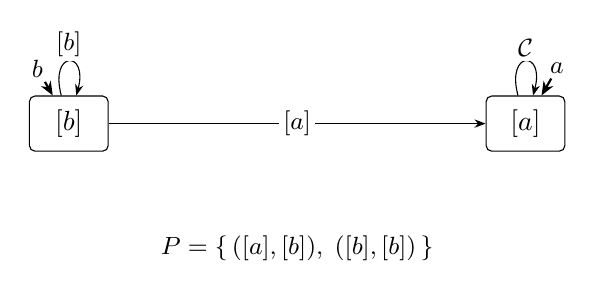
\begin{tikzpicture}[
  class/.style     = {draw, thin, rounded corners=2pt, inner sep=3pt,
                      minimum width=10mm, minimum height=7mm},
  root/.style      = {},          % the root needs no ink: the init stub says it
  init/.style      = {semithick, -{Stealth[length=4pt,width=3pt]}},
  lstub/.style     = {thick, -{Stealth[length=5pt,width=4pt]}},
                       % a lambda stub: heavier than init, it is a stub not a node
  arrow/.style     = {thin, -{Stealth[length=4pt,width=3pt]}},
  pair/.style      = {very thick, double, double distance=1pt,
                      -{Stealth[length=6pt,width=5pt]}},
                       % an accepting pair (s,e) drawn as a bold doubled loop at s
  lbl/.style       = {font=\small, inner sep=1.5pt, fill=white,
                      align=center},   % a long class list wraps (see WRAP_CHARS)
  letters/.style   = {font=\small, inner sep=1.5pt, align=center},
                       % the source letters of a lambda stub: no brackets, math italic
  pairs/.style     = {anchor=north, font=\small},
]

  \node[class] (a) at (6.8,0.6) {$[a]$};
  \node[class] (b) at (1.0,0.6) {$[b]$};

  % λ: the letters naming each class, entering it as a source (no brackets — a letter is not a class)
  \node[letters] (lam_a) at (7.2,1.3) {$a$};
  \draw[lstub] (lam_a) -- (a);
  \node[letters] (lam_b) at (0.6,1.3) {$b$};
  \draw[lstub] (lam_b) -- (b);

  \draw[arrow] (a) to[loop above] node[lbl] {$\mathcal{C}$} (a);
  \draw[arrow] (b) to node[lbl] {$[a]$} (a);
  \draw[arrow] (b) to[loop above] node[lbl] {$[b]$} (b);

  \node[pairs] at (3.9,-0.7) {$P = \{\, ([a],[b]),\; ([b],[b]) \,\}$};
\end{tikzpicture}
\end{document}
